% !TeX root = chapter02.tex
\documentclass[
    ngerman,
    accentcolor=3b,
    % dark_mode, % uncomment for dark mode
    fontsize= 12pt,
    a4paper,
    aspectratio=169,
    colorback=true,
    fancy_row_colors,
    leqno,
    fleqn,
    boxarc=3pt,
    fleqn,
    main,
    design=2008,
    % shell_escape = false, % Kompatibilität mit sharelatex
]{algoslides}
\RequirePackage{import}
\subimport{../common}{preamble}

%%--------------------------%%
%%--Imports from Main File--%%
%%--------------------------%%

% Get Labels from Main Document using the xr-hyper Package
\externaldocument[ext:]{../main}
% Set Graphics Path, so pictures load correctly
\graphicspath{{../pictures}}

\begin{document}
    \section{Demonstration}\label{2}\label{Demonstration}
    \begin{frame}[<+(1)->]
        \slidehead{}
        \boldimpact{Demonstration}
    \end{frame}

    \begin{frame}
        \slidehead{}
        \vspace{-1em}
        \begin{columns}[c]
            \begin{column}{.5\textwidth}
                \begin{figure}[ht!]
                    \centering
                    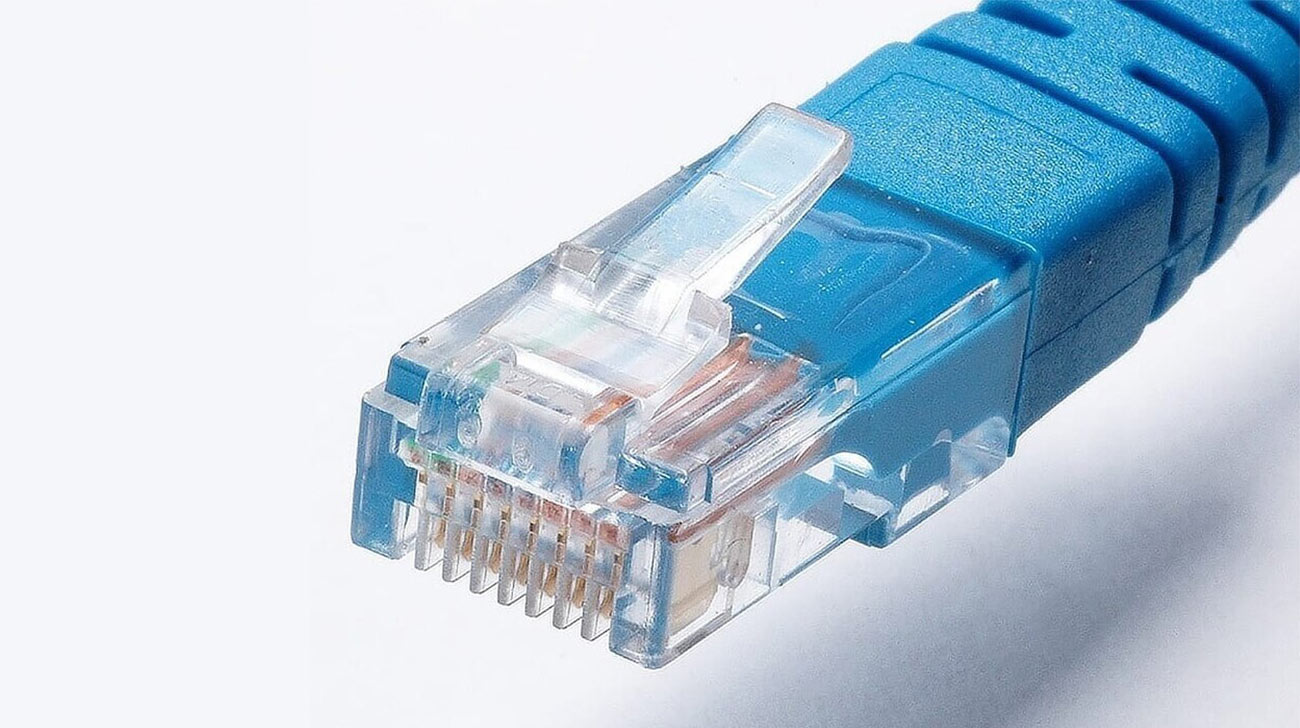
\includegraphics[height=.3\textheight]{rj45-plug}
                    \label{fig:rj45-plug}

                    \vspace{1em}
                    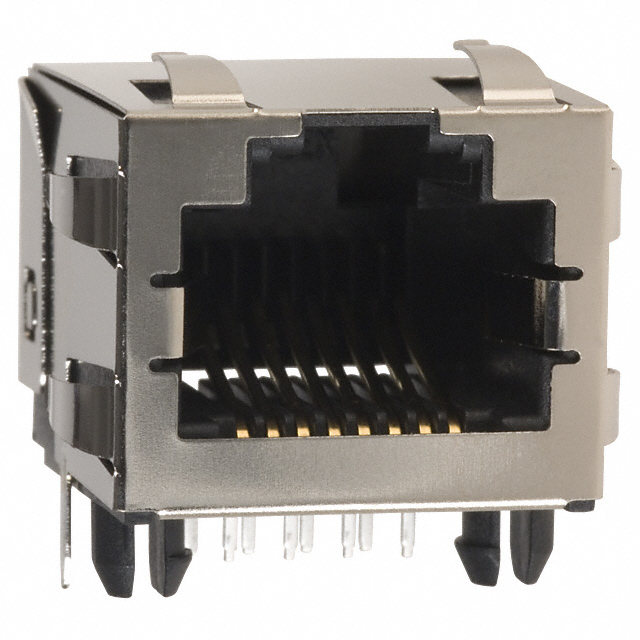
\includegraphics[height=.3\textheight]{rj45-socket}
                    \label{fig:rj45-socket}
                \end{figure}
            \end{column}
            \pause
            \begin{column}{.5\textwidth}
                \large
                \centering
                RJ45
            \end{column}
        \end{columns}
    \end{frame}

    \begin{frame}
        \slidehead{}
        \vspace{-1em}
        \begin{columns}[c]
            \begin{column}{.5\textwidth}
                \begin{figure}[ht!]
                    \centering
                    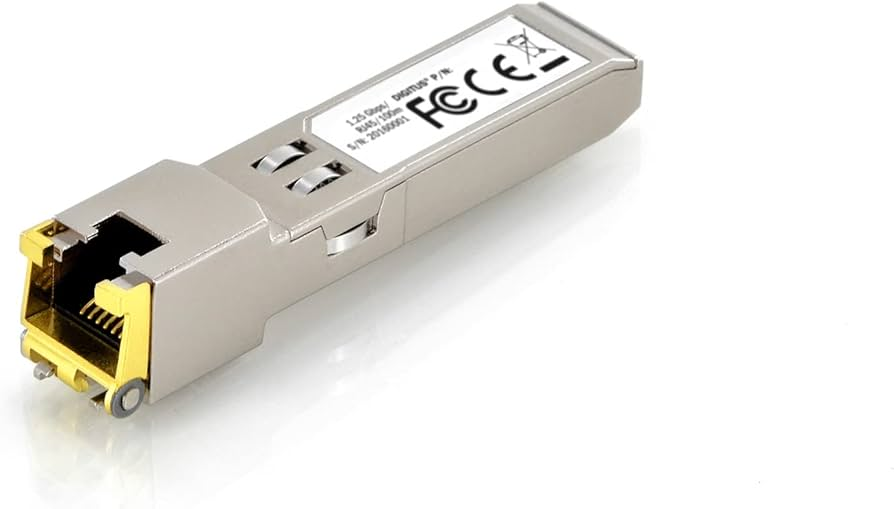
\includegraphics[height=.3\textheight]{sfp-rj45}
                    \label{fig:sfp-rj45}

                    \vspace{1em}
                    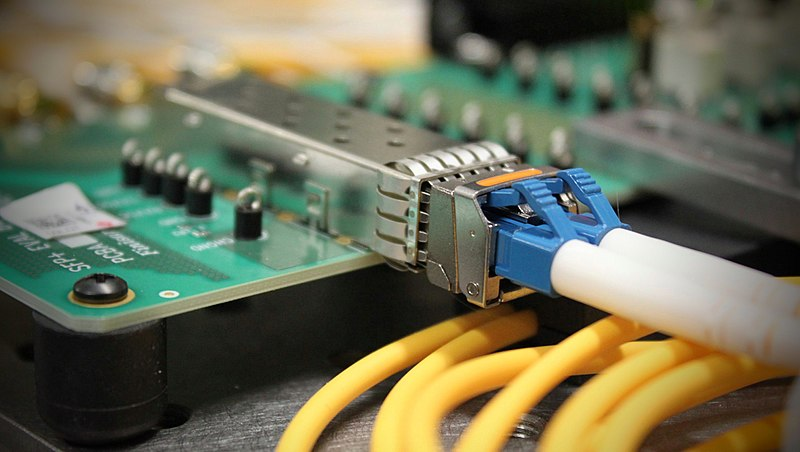
\includegraphics[height=.3\textheight]{sfp-socket}
                    \label{fig:sfp-socket}
                \end{figure}
            \end{column}
            \pause
            \begin{column}{.5\textwidth}
                \large
                \centering
                SFP
            \end{column}
        \end{columns}
    \end{frame}

    \begin{frame}
        \slidehead{}
        \vspace{-1em}
        \begin{columns}[c]
            \begin{column}{.5\textwidth}
                \begin{figure}[ht!]
                    \centering
                    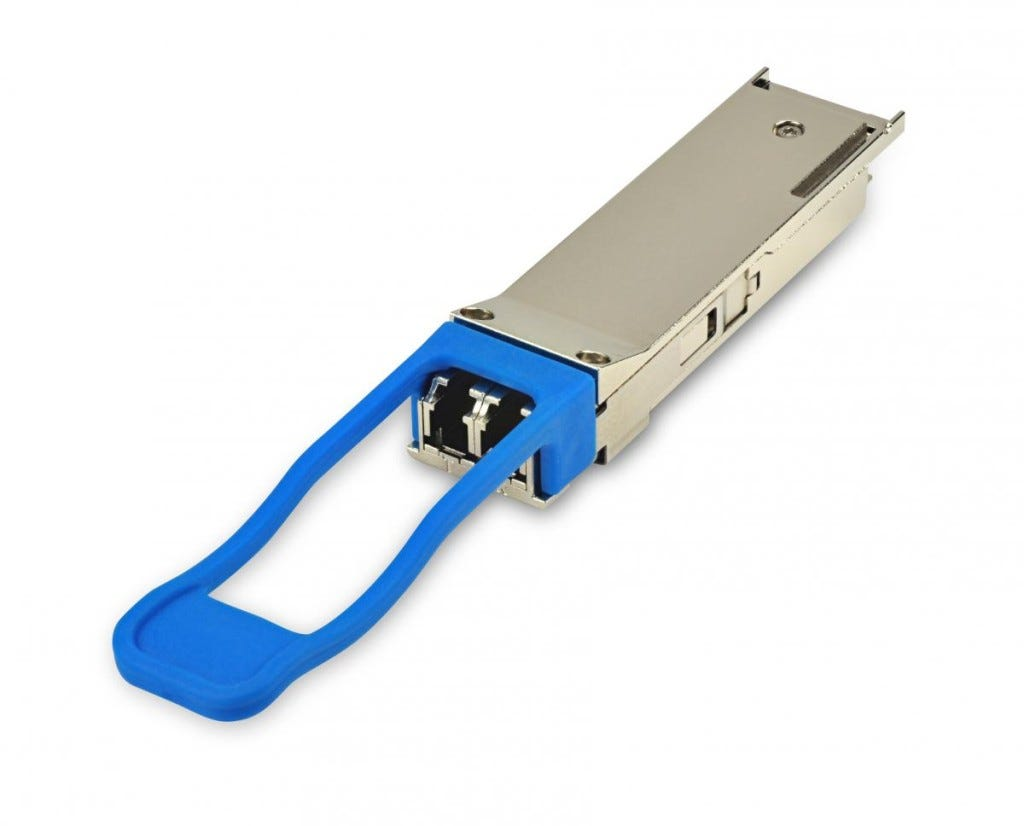
\includegraphics[height=.6\textheight]{qsfp-transciever}
                    \label{fig:qsfp-transciever}
                \end{figure}
            \end{column}
            \pause
            \begin{column}{.5\textwidth}
                \large
                \centering
                QSFP
            \end{column}
        \end{columns}
    \end{frame}

\end{document}
